%-------------------------------------------------------------------------------
% BIFURCATION ANALYSIS 
%-------------------------------------------------------------------------------

\section{Bifurcation Analysis and Dynamical Systems} \label{sec:bif}

Hydrodynamic stability theory studies how a fluid flow is affected by small
disturbances of an initial state. This analysis involves analytical,
experimental, and more and more computational explorations. Flow regimes can be
categorized as either linearly unstable or stable. Unstable in the sense that
even infinitesimal variations will cause the flow to deviate from its initial
state, resulting in a different flow state or the onset of turbulence.
Conversely, disturbances do not change the initial system's state in a stable
flow. In the context of the R4CF problem, the objective is to investigate the
flow arising in the driven cavity for different configurations through
numerical computations. We want to mainly understand how the flow is affected
by the length of the side walls, the boundary velocity, and the fluid's
viscosity, all of these quantities captured by the Reynolds number.

In figure \ref{fig:timestepping}, it has been identified that two asymmetric
states are possible when the Reynolds number exceeds a critical threshold, and
although the symmetric base flow remains a solution to the governing equations,
it becomes unstable. The point at which the two states emerge is called a
bifurcation point. A bifurcation is the change of a value of qualitative
character of the set of possible steady and unsteady flows in dynamical
equilibrium \citep{drazin2002}. These points are often associated with
instabilities, multiple flow patterns, or the emergence of oscillatory
behavior. We recall the original bifurcation diagram presented in figure
\ref{fig:bif_diag_chen}. To understand this diagram and to differentiate the
points where the flow states are altered, we want to introduce the mathematical
underpinnings from a dynamical system point of view. After that, the occurring
bifurcations for the R4CF will be explained in detail.

\subsection{The Dynamical Systems Perspective}

An alternative perspective on our problem at hand is through the theory of
dynamical systems:
\begin{align}
  \frac{dx}{dt} = {f(x, \mu)}, \label{eq:dyn_sys_orig}
\end{align}
where $x$ represents a state variable and $\mu$ is a parameter. In this
framework $x$ is a multidimensional point within a set of all possible states
referred to as the state space or phase space (indicated as $X$). This point
describes the system's current state and includes all the necessary dimensions
to determine its future evolution.

The solution $x(t)$ depends on a time variable $t \in T$, where $T$, in our
case, is a set of positive real numbers ($T \in \mathbb{R}^+$). We can define
an evolution operator $\varphi_t : X \to X$, which is a map that describes the
system's transformation over time. Formally, a dynamical system is written as a
triple $\{ T, X, \varphi^t \}$ \citep{kuznetsov2004}.

The equation of the streamfunction \eqref{eq:str} is an autonomous partial
differential equation, which can be reformulated as a dynamical system. We
consider an infinite-dimensional point denoted as $\Psi$ in a state space $X$.
$\Psi$ can be thought of as a vector covering all possible points of our cavity
and thus is infinite-dimensional. Using the streamfunction at time $t$, we have
not only the locations of all fluid particles but also their evolution
(velocities $u$ and $v$) explicitly given by the definition of the derivatives
\eqref{eq:str_defx} and \eqref{eq:str_defy}.

Further, this infinite-dimensional space will be divided into discrete points
with the chosen pseudo-spectral discretization. Increasing the number of
Chebyshev grid points $m$ and $n$ should result in higher accuracy and the
solution is expected to converge exponentially because of the
singularity-avoiding regularization. The finite-dimensional space for the
numerical computations can be defined as:
\begin{align}
  \frac{d\Psi_j}{dt} &= {F_j(\Psi, \Rey)}, \quad \quad \quad
    j= 1,2,\dots,(m+1)(n+1), \label{eq:dyn_sys}
\end{align}

where $F_j$ is the $j$-th component of the nonlinear function at the $j$-{th}
grid point. Equations \eqref{eq:dyn_sys} is essentially a dynamical system of
$(m+1)(n+1)$ equations, and one parameter, namely the Reynolds number $\Rey$.

This more abstract framework is helpful in the sense that it provides a
geometrical representation of the sought-after solutions. It is useful to look
at subsets of the phase space $X$. Of particular interest are the so-called
invariant sets, subsets $S$ satisfying $\varphi_t(S) \in S$ for all $t \in T$.
If $S$ is just one single point, having measure $0$, this set is called a fixed
point (or equilibrium). One-dimensional invariant manifolds may also be
dynamically relevant. An example is an isolated periodic orbit (or limit cycle)
which is a closed trajectory such that there exists a time $T > 0$ for which
$\varphi_{t+T}(x) = \varphi_{t}(x)$. A stable periodic orbit corresponds to a
closed trajectory, where other nearby trajectories converge toward the orbit.
An unstable periodic orbit is characterized by nearby trajectories diverging
away from it. Further, periodic orbits can be classified by their period and
amplitude and are usually depicted in what is called a phase portrait.
Equilibria and periodic orbits interact, leading to homoclinic connections,
which are one-dimensional sets of self-connected equilibria. If an orbit
reconnects more than one equilibrium, it is called a heteroclinic connection
\citep{kuznetsov2004}.

These invariant sets help to characterize dynamical systems and understand the
fundamental types of solutions when a parameter of interest is varied.


\subsection{Steady-State Flows}

We have seen that launching a time stepper gives different kinds of states
depending on the initial condition. A steady-state solution corresponds to a
solution of the differential equation where the time $t$ approaches infinity,
satisfying
\begin{align}
  F(\Psi, \Rey) &= \frac{1}{\Rey}\Delta^2 \Psi +
    (\partial_x \Psi) \partial_y(\Delta \Psi) -
    (\partial_y \Psi) \partial_x(\Delta \Psi) \nonumber \\
  & =  0, \quad \text{or} \\
  F_j(\Psi, \Rey) &= 0, \quad \quad \quad 
  j= 1,2,\dots,(m+1)(n+1), \label{eq:str_steady}
\end{align}

in the discretized version. As the outer two grid rows and columns are
explicitly known through the boundary conditions (explained in section
\ref{sec:bc}), a reduced system of equations $F(\psi, \Rey) = 0$, can be
formulated, where $\psi \in \mathbb{R}^{(m-1)\times(n-1)} $ corresponds now to
the inner grid points. Thus, in practice, the system is
$(m-1)(n-1)$-dimensional and solvable with Newtons's method.

\subsection{Linear Stability Analysis}

To analyze the stability of steady flows converged with Newton's method, we
perform a linear stability analysis. Given an equilibrium solution $\Psi_0$,
satisfying equation \eqref{eq:str_steady}, we perturb it by adding a small
disturbance
\begin{align}
\Psi = \Psi_0 + \epsilon \tilde{\Psi},
\end{align}

where $\epsilon$ is a small amplitude, and $\tilde{\Psi}$ is and arbitrary
field satisfying homogeneous boundary conditions. We can insert this expression
into the time-dependent streamfunction equation \eqref{eq:str}. By only
identifying first-order terms $\mathcal{O}(\epsilon)$ and using the fact that
$F_{steady}(\Psi_0) = 0$, we get,
\begin{align}
\partial_t \Delta \tilde{\Psi} = \frac{1}{Re} \Delta^2 \tilde{\Psi}
  + (\partial_x \Psi_0) \partial_y (\Delta \tilde{\Psi})
  + (\partial_x \tilde{\Psi}) \partial_y (\Delta \Psi_0)
  - (\partial_y \Psi_0) \partial_x (\Delta \tilde{\Psi})
  - (\partial_y \tilde{\Psi}) \partial_x (\Delta \Psi_0).
\label{eq:str_pert}
\end{align}

To solve this linear stability analysis problem, an ansatz is used, where we
separate time and the spatial variables as follows: 
\begin{align}
  \tilde{\Psi} = \tilde{\Psi}(x,y,t) = \mathrm{e}^{\lambda t} \Phi(x,y),
  \label{eq:ansatz}
\end{align}

where $\Phi$ is the eigenfunction associated with the eigenvalue $\lambda$,
whose real part will dictate the stability or instability of $\Psi_0$. After
formal substitution of the ansatz \eqref{eq:ansatz} into \eqref{eq:str_pert},
the exponential time dependence of the problem disappears, leading to an
algebraic generalized boundary eigenvalue problem that reads
\begin{align}
\lambda \Delta \Phi = \frac{1}{Re} \Delta^2 \Phi
  + (\partial_x \Psi_0) \partial_y (\Delta \Phi)
  + (\partial_x \Phi) \partial_y (\Delta \Psi_0)
  - (\partial_y \Psi_0) \partial_x (\Delta \Phi)
  - (\partial_y \Phi) \partial_x (\Delta \Psi_0),
\label{eq:str_phi}
\end{align}

where $\Phi = 0$ at the boundaries. In terms of two operators $A$ and $B$,
the problem can be stated as follows: 
\begin{align} \label{eq:eig_prob}
  \begin{split}
  A \Phi & = \lambda B \Phi \\[4pt]
  \begin{split}
  A & = \frac{1}{Re} \Delta^2 \bullet
    + (\partial_x \Psi_0) \partial_y (\Delta \bullet)
    + (\partial_x \bullet) \partial_y (\Delta \Psi_0) \\
    &\quad - (\partial_y \Psi_0) \partial_x (\Delta \bullet)
    - (\partial_y \Phi) \partial_x (\Delta \Psi_0)
  \end{split} \\
  B & = \Delta
  \end{split}
\end{align}

We recognize that $\Phi(x,y)$ corresponds to an eigenmode, and $\lambda$ is the
associated eigenvalue. If all the eigenvalues of the generalized eigenvalue
problem have a positive real part, the equilibrium is stable. On the contrary,
if only one of the eigenvalues is found to be positive, then the system is
unstable because a small perturbation will grow exponentially in time, which
can be directly seen in the definition of the ansatz.

This linear stability problem becomes computationally demanding because the
perturbation $\Phi$ acts on every grid point, and the numerical eigenvalue
problem is solved with matrices of the size $(m+1)(n+1) \times (m+1)(n+1)$. We
compute the whole spectrum of eigenvalues using the QZ algorithm (\jlinl{eigen}
function in Julia). The Arnoldi
method employed for a partial evaluation of the spectrum has been tried but
did not converge in the case of the R4CF.

A final remark is that with linear stability analysis, we only look at linear
perturbation, meaning that nonlinear disturbances (second or higher order) are
not captured with this technique.

\subsection{Bifurcations} \label{sec:bif_details}

We have formally defined the tools needed to characterize all the bifurcations
occurring in the RCF4 precisely. 

To illustrate the bifurcations we encountered, a parameter of interest $\mu$
($\Rey$ in the R4CF) will be varied and plotted against a variable that
identifies different states. Lets denote this variable by $U$ ($\Psi_{center}$
in the R4CF). The first bifurcation we want to look at is a pitchfork (figure
\ref{fig:pitch_saddle}), where the symmetry of the problem is broken, and two
different flow solutions appear. The base solution is still an equilibrium but
linearly unstable for $\mu > \mu_c$.

\begin{figure}[ht]
\centering
\begin{subfigure}[t]{0.3\textwidth}
  \centering
  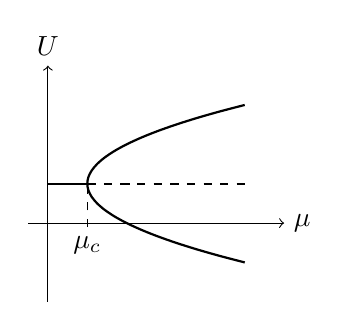
\begin{tikzpicture}[scale=0.5]
    \draw[->] (-0.5,0) -- (6,0) node[right] {$\mu$};
    \draw[->] (0,-2) -- (0,4) node[above] {$U$};
    
    \draw[thick] plot[smooth,domain=-2:2] ({1 + \x*\x},1 + \x);
    \draw[thick] plot[smooth,domain=0:1] (\x,1);
    \draw[thick] plot[smooth,domain=0:1] (\x,1);

    \draw[thick, dashed] plot[smooth,domain=1:5.2] (\x,1);
    
    \draw[dashed] (1,-0.1) -- (1,1);
    \node[below] at (1,-0.1) {$\mu_c$};
  \end{tikzpicture}
\end{subfigure}
\hspace{0.1\textwidth}
\begin{subfigure}[t]{0.3\textwidth}
  \centering
  \begin{tikzpicture}[scale=0.5]
    \draw[->] (-0.5,0) -- (6,0) node[right] {$\mu$};
    \draw[->] (0,-2) -- (0,4) node[above] {$U$};

    \draw[thick, dashed] plot[smooth,domain=-1.9:0] ({5 - 1.2*\x*\x},1 + \x);
    \draw[thick] plot[smooth,domain=0:1.9] ({5 - 1.2*\x*\x}, 1 + \x);

    \draw[dashed] (5,-0.1) -- (5,1);
    \node[below] at (5,-0.1) {$\mu_c$};
  \end{tikzpicture}
\end{subfigure}
\caption{Supercritical pitchfork bifurcation (left) and a saddle-node (right)}
  \label{fig:pitch_saddle}
\end{figure}

Another type of bifurcation is called a saddle-node or fold bifurcation, where
a set of stable and unstable fixed points collide at $\mu = \mu_c$. See the
bifurcation diagram shown in figure \ref{fig:pitch_saddle} to the right.

Finally, a Hopf bifurcation is characterized by a complex conjugate pair of
eigenvalues crossing the imaginary axis at some critical value $\mu = \mu_c$.
At a Hopf bifurcation, a stable fixed point becomes unstable, and the system
starts to oscillate. A sketch of the amplitudes is depicted in figure
\ref{fig:hopf}. One can distinguish between sub- and supercritical Hopf
bifurcations. In the supercritical case, the system is changing suddenly from a
fixed point to a stable periodic orbit (SPO). On the other hand, the
subcritical Hopf is less predictable. Before the critical $\mu$, there are
unstable periodic orbits (UPO), and then it is unclear what happens when the
fixed point becomes unstable.

\begin{figure}[ht]
\centering
\begin{subfigure}[t]{0.3\textwidth}
  \centering
  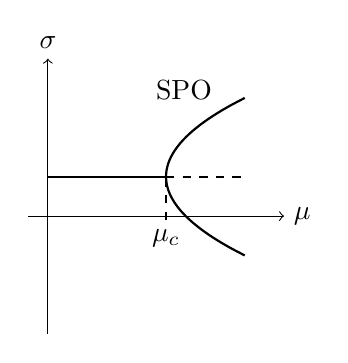
\begin{tikzpicture}[scale=0.5]
    \draw[->] (-0.5,0) -- (6,0) node[right] {$\mu$};
    \draw[->] (0,-3) -- (0,4) node[above] {$\sigma$};
    
    \draw[thick] plot[smooth,domain=-2:2] ({3 + 0.5*\x*\x},1 + \x);
    \draw[thick] plot[smooth,domain=0:3] (\x,1);
    \draw[thick] plot[smooth,domain=0:3] (\x,1);

    \draw[thick, dashed] plot[smooth,domain=3:5] (\x,1);
    \draw[thick, dashed] plot[smooth,domain=3:5] (\x,1);
    
    \draw[dashed] (3,-0.1) -- (3,1);
    \node[below] at (3,-0.1) {$\mu_c$};

    \node[above right] at (2.5,2.7) {SPO};
  \end{tikzpicture}
\end{subfigure}
\hspace{0.1\textwidth}
\begin{subfigure}[t]{0.3\textwidth}
  \centering
  \begin{tikzpicture}[scale=0.5]
    \draw[->] (-0.5,0) -- (6,0) node[right] {$\mu$};
    \draw[->] (0,-3) -- (0,4) node[above] {$\sigma$};

    \draw[thick, dashed] plot[smooth,domain=-2.1:2.1] ({3 - 0.5*\x*\x},1 + \x);
    \draw[thick] plot[smooth,domain=0:3] (\x,1);
    \draw[thick] plot[smooth,domain=0:3] (\x,1);

    \draw[thick, dashed] plot[smooth,domain=3:4.8] (\x,1);
    \draw[thick, dashed] plot[smooth,domain=3:4.8] (\x,1);
    
    \draw[dashed] (3,-0.1) -- (3,1);
    \node[below] at (3,-0.1) {$\mu_c$};

    \node[above right] at (1.4,2.7) {UPO};
  \end{tikzpicture}
\end{subfigure}
\caption{Sketch of amplitudes of stable (SOP) and unstable (UPO) periodic orbits
  for supercritical (left) and subcritical Hopf (right)}
\label{fig:hopf}
\end{figure}

\subsection{Continuation Algorithms} \label{sec:cont}

The next key idea is how to track branches of steady flows. The simplest
numerical algorithm is called natural continuation, where we start with a
solution obtained by a time-stepper or the Newton algorithm and then increase
the Reynolds number. The initial guess for the next Newton iteration is the
solution of the step before. In this way, we can "continue" a branch without
using a time integration algorithm for each steady-state solution we want to
obtain. The Newton method will converge if the steps in $\mu$ are small enough.
Furthermore, unstable branches can be followed as well, which can not be done
solely by time evolution.

However, there is a limitation. In the fold bifurcation depicted in figure
\ref{fig:pitch_saddle}, the continuation has to follow a curve when the
parameter is decreasing again. The natural continuation cannot properly achieve
this, as the Reynolds number is manually set to increase. Another strategy to
overcome this issue is called pseudo-arclength continuation
\citep{kuznetsov2004}. Given two fixed points $x^{(0)}$ and $x^{(1)}$ on a
curve with parameter values $\mu^{(0)}$ and $\mu^{(1)}$, we want to find the
next $x^{(2)}$ and $\mu^{(2)}$ making a prediction with the approximated
tangents from the already given fixed points:
\begin{equation}
  \tilde{x}^{(2)} = x^{(1)}  + \underbrace{[x^{(1)} - x^{(0)}]}_{\text{\normalfont $\hat{x}$}} \gamma
\end{equation}

Here $\gamma$ (in this study set to $1$) is a parameter that determines the
prediction step size. $\tilde{x}^{(2)}$ is called the predictor. Now, another
equation is imposed, which is referred to as the correction step:
\begin{equation}
  (x^{(2)} - x^{(1)})  \cdot \hat{x} = 0 \label{eq:extra}
\end{equation}

This equation tells us that we want to find the next point on the curve, that
is orthogonal to the tangent drawn from our previous points. Figure
\ref{fig:pseudo_cont} illustrates this idea geometrically. Consequently,
$\mu^{(2)}$ is determined explicitly by satisfying the equation
\eqref{eq:extra}. To find the next point, the initial system of nonlinear
equations \eqref{eq:dyn_sys} is augmented by
\begin{equation}
  F(x^{(2)}, \mu^{(0)}) = 
\begin{bmatrix} F(x^{(2)}, \mu) \\ (x^{(2)} - x^{(1)})  \cdot \hat{x}
\end{bmatrix}, \label{eq:dyn_sys_cont}
\end{equation}

which means the parameter $\mu$ is now part of the equation. The augmented
Jacobian can be formulated as follows: 
\begin{equation}
\renewcommand\arraystretch{1.5}
J = 
\left[
\begin{array}{cc}
  J_x \quad \quad \quad \quad & F_{\mu} \\
  \hdashline
  \quad (x^{(2)} - x^{(1)})^T
\end{array} \label{eq:jac_aug}
\right]
\end{equation}

First of all, we calculate the original Jacobian $J_x$. The components
of the last row of the augmented Jacobian are given by the transpose of the
distance in phase space between the two already computed states. The last
column (excluding the last row) corresponds to the finite difference derivative
of the nonlinear function with respect to $\mu$. It is necessary to scale the
parameter $\mu$ to obtain changes with similar magnitudes as for the $x$
components. This ensures a well-conditioned Jacobian.

\begin{figure}[h]
\centering
\begin{tikzpicture}
  \draw[->] (0,-0.5) -- (0,4) node[above] {$"x"$};
  \draw[->] (-0.5,0) -- (4,0) node[right] {$\mu$};

  \draw[smooth, thick, variable=\x, domain=0.5:4] plot ({\x},{2 - 0.25*(\x - 2.5)^2});

  \draw[fill=black] (0.6,{2 - 0.25*(0.6 - 2.5)^2}) circle (0.05) node[below] {$x^{(0)}$};
  \draw[fill=black] (1.2,{2 - 0.25*(1.2 - 2.5)^2}) circle (0.05) node[below] {$x^{(1)}$};

  \draw[dashed] (0.6,{2 - 0.25*(0.6 - 2.5)^2}) -- (2.5,{0.6 + ((2 - 0.25*(1.2 - 2.5)^2) - (2 - 0.25*(0.6 - 2.5)^2))/0.6*2.5});

  \draw[dashed] ((2.5,{0.6 + ((2 - 0.25*(1.2 - 2.5)^2) - (2 - 0.25*(0.6 - 2.5)^2))/0.6*2.5}) -- (3,{2 - 0.25*(3 - 2.5)^2});

  \draw[fill=black] ((2.5,{0.6 + ((2 - 0.25*(1.2 - 2.5)^2) - (2 - 0.25*(0.6 - 2.5)^2))/0.6*2.5}) 
    circle (0.05) node[above] {$\tilde{x}^{(2)}$};;
  \draw[fill=black] (3,{2 - 0.25*(3 - 2.5)^2}) circle (0.05) node[below] {$x^{(2)}$};;
\end{tikzpicture}
\caption{Pseudo-arclength continuation, a simplified illustration by projecting the vector $x$ on a plane}
\label{fig:pseudo_cont}
\end{figure}
